\section{The star skeleton}\label{sec:star}
Let $o$ be the central branch vertex and $u_1,u_2,u_3$ the three terminal branch vertices, with connector lengths $L_1,L_2,L_3\ge1$. The center may have no side arms. Write $E_c$ for its product of equal-length arm pairs, so $0\le E_c\le1$.

\subsection{The center catalogue}
The residual center tables fall into three classes. In the first, a fixed message $C$ satisfies
\begin{equation}\label{eq:center3}
 \E[q^3C^4]\le1.
\end{equation}
The table gives the direction for each row. The factor $E_c$ multiplies every row, and the products $P$ and $V^+$ involve only the indicated residual arms.

\begin{table}[htbp]
\centering
\caption{Center directions with a cubed-weight fourth moment.}\label{tab:center}
\fontsize{9}{11}\selectfont
\setlength{\tabcolsep}{1pt}\noindent\begin{tabular}{@{}p{56mm}p{66mm}p{32mm}@{}}
\toprule
Residual center table & Message $C/E_c$ & Complete proof\\\midrule
Singleton $a\ge1$ & $f_a$ & Section~\ref{loc:S36}\\
Odd, at least three, minimum one & $pP$, $P$ canonical on the rest & Section~\ref{loc:S18}; \eqref{eq:unitcenter}\\
Odd, at least three, minimum $a\ge2$ & $f_aP$, $P$ canonical on the rest & Section~\ref{loc:S18}\\
Even, minimum two & $f_2h_{b_1}\prod_{i=2}^t h_{a_i}f_{b_i}$ & Section~\ref{loc:S38}\\
Even, minimum three & $f_3h_{b_1}\prod_{i=2}^t h_{a_i}f_{b_i}$ & Section~\ref{loc:S37}\\
Even, minimum at least four & $\prod_{i=1}^t h_{a_i}f_{b_i}$ & Section~\ref{loc:S37}\\
Even, at least four, minimum one & $pV^+$ & Section~\ref{loc:S38}; \eqref{eq:unitcenter}\\
\bottomrule
\end{tabular}

\end{table}

The unit-arm reductions in the second and last rows are direct. If $V\ge0$ is the message of the row in question, with $\E[pV^4]\le1$, then
\begin{equation}\label{eq:unitcenter}
 \E[q^3(pV)^4]=\E[p(pq)^3V^4]\le\E[pV^4]\le1.
\end{equation}
For an odd center of minimum one, $V=P$ is the canonical even product. For an even center with at least four entries and minimum one, the remaining odd list has at least three entries, and $V^+$ is exactly its zero-step direction in \eqref{eq:zeroOdd}. The leading $p$ comes from the unit arm.

The singleton row directs its residual arm outward for every length and is proved in
Section~\ref{loc:S36}, with a separate certificate for the two-edge arm.

The second center class consists of a residual list exactly $(1,b)$, $b\ge2$. Direct both residual arms outward and take
\begin{equation}\label{eq:center9}
 C=E_cpf_b,\qquad
 \E[q^9C^4]\le\E[q^5f_b^4]\le1.
\end{equation}
Indeed $q^9C^4=E_c^4(pq)^4q^5f_b^4$. The last inequality is the complete singleton estimate in Sections~\ref{loc:S17}, \ref{loc:S19}. This class uses the ninth power rather than the cubed weight, including the case $b=2$.

The third class has an empty residual list and message $C=E_c\le1$; Section~\ref{sec:emptystar} handles it with a different merger.

The first class
contains every odd nonempty list and every even list whose minimum is two,
three, or at least four. An even list with minimum one has either two
entries, which gives the second class, or at least four, which gives the
first. The empty list is the third class.

\begin{figure}[htbp]\centering
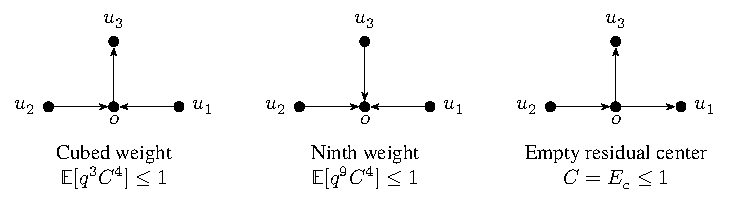
\includegraphics{figures/star-centers.pdf}
\caption{Core directions for the three star-center constructions. The empty-center case uses a full $L_1$-step terminal on the right-hand path and a second-moment terminal on the upper path. All connector lengths remain positive and arbitrary.}\label{fig:star}
\end{figure}

\subsection{Cubed-weight centers: two incoming paths and one outgoing path}
Assume \eqref{eq:center3}. Reducible terminals have already been covered by Lemma~\ref{lem:reduction}. Fix the core directions
\[
 u_1\longrightarrow o,\qquad u_2\longrightarrow o,
 \qquad o\longrightarrow u_3,
\]
with every original edge of each path pointing consistently. Put
\[
 G_i=T^{L_i-1}F^+_{i,L_i-1}\quad(i=1,2),\qquad
 H_3=A^{L_3-1}F^-_{3,L_3-1}.
\]
The terminal theorem gives $\E[pG_i^4]\le1$ and $\E[qH_3^4]\le1$. Retaining only the final edge near $o$ on each path, the density is
\begin{equation}\label{eq:stardensity}
 Z_D=\E[C(TG_1)(TG_2)(AH_3)].
\end{equation}
We control two groups at the same center label. First,
\begin{align}
 \norm{CTG_1}_2^2
 &\le\E[qC^2T(G_1^2)]\notag\\
 &\le\sqrt{\E[q^3C^4]\,\E[pG_1^4]}\le1.\label{eq:starfirst}
\end{align}
The first step is row Cauchy--Schwarz; the second applies Cauchy--Schwarz to the $T$ edge measure, whose root marginal is $q\mu$.
For the other two paths, row Cauchy--Schwarz and $pq\le1$ give
\begin{align}
 \norm{(TG_2)(AH_3)}_2^2
 &\le\E[pq\,T(G_2^2)A(H_3^2)]\notag\\
 &\le\ip{G_2^2}{A^2(H_3^2)}\notag\\
 &\le\sqrt{\E[pG_2^4]\,\E[qH_3^4]}\le1.\label{eq:starsecond}
\end{align}
The middle expression uses $T^*=A$, and the last step is Lemma~\ref{lem:connector} with length two. The joint estimate integrates the two adjacent edges at their common label. Applying ordinary Cauchy--Schwarz to the two groups in \eqref{eq:stardensity} proves $Z_D\le1$.

\subsection{Ninth-weight centers: all three paths incoming}
Now use \eqref{eq:center9} and direct every connector from $u_i$ toward $o$. Set $G_i=T^{L_i-1}F^+_{i,L_i-1}$, so $\E[pG_i^4]\le1$. The exact density is
\[
 Z_D=\E\left[C\prod_{i=1}^3TG_i\right].
\]
H\"older on a row of the nonnegative $T$ kernel gives
\begin{equation}\label{eq:rowholder}
 (TG_i)^4\le q^3T(G_i^4).
\end{equation}
The factor $q^3$ reflects the mass $q$ of the row measure. Apply \eqref{eq:rowholder}, followed by four-factor H\"older on the original probability measure:
\begin{align*}
 Z_D&\le\E\left[Cq^{9/4}\prod_{i=1}^3T(G_i^4)^{1/4}\right]\\
 &\le\left(\E[q^9C^4]\prod_{i=1}^3\E[T(G_i^4)]\right)^{1/4}\\
 &=\left(\E[q^9C^4]\prod_{i=1}^3\E[pG_i^4]\right)^{1/4}\le1.
\end{align*}
The equality uses $\E[Tv]=\E[pv]$.

\subsection{Empty residual center}\label{sec:emptystar}
Here $C=E_c\le1$. Choose the core directions $o\to u_1$, $u_2\to o$, and $o\to u_3$. At the first terminal use the \emph{positive-step} supply through the entire first path:
\[
 X=A^{L_1}F^-_{1,L_1},\qquad \E[qX^4]\le1.
\]
At the second terminal retain its last edge and put
\[
 G=T^{L_2-1}F^+_{2,L_2-1},\qquad \E[pG^4]\le1.
\]
At the third terminal choose the actual spider direction of Lemma~\ref{lem:spidersecond}, with message $F_3$ and $N_-(F_3)\le1$; a second-moment bound suffices here.

Let $H=X(TG)$. Row Cauchy--Schwarz, followed by edge Cauchy--Schwarz with the correct marginals, yields
\begin{align*}
 N_+(H)&\le\E[pqX^2T(G^2)]\\
 &\le\sqrt{\E[p^2q^3X^4]\,\E[pG^4]}\\
 &\le\sqrt{\E[qX^4]\,\E[pG^4]}\le1.
\end{align*}
In the last comparison $p^2q^2\le1$ is used. Multiplying by $C\le1$ gives $N_+(CH)\le1$. The exact density is
\[
 Z_D=\ip{CH}{A^{L_3}F_3}
 \le\sqrt{N_+(CH)N_-(F_3)}\le1.
\]
The three center constructions, the terminal catalogue, and Lemma~\ref{lem:reduction} prove the assertion for the $K_{1,3}$ skeleton.
